\documentclass[10pt]{article}
\usepackage[utf8]{inputenc}
\usepackage[myheadings]{fullpage}
\DeclareUnicodeCharacter{0301}{\hspace{-1ex}\'{ }}
% Package for headers 
\usepackage{fancyhdr}
\usepackage{lastpage}
\usepackage{listings}

% For figures and stuff
\usepackage{graphicx, wrapfig, subcaption, setspace, booktabs}
\usepackage[T1]{fontenc}
\usepackage{array}
\usepackage{longtable}
\usepackage{rotating}
\newcommand*\rot{\rotatebox{90}}

% Change for different font sizes and families
\usepackage[table,xcdraw]{xcolor}

% Maths
\usepackage{amsmath,amssymb}
\usepackage{float}
\usepackage{graphicx}
\usepackage{wrapfig}
\usepackage[colorinlistoftodos]{todonotes}
\usepackage[colorlinks=true, allcolors=blue]{hyperref}
\usepackage[super]{nth}
\usepackage{tikz}
\usetikzlibrary{automata, positioning}


%Grammar expression
\usepackage[altpo]{backnaur}

% Bibliography
\usepackage[
    sorting=none,
	backend=biber
]{biblatex} 
\addbibresource{bibliography.bib}

%% Language and font encodings
\usepackage[english]{babel}
\usepackage{csquotes}
\usepackage{titlesec}

\usepackage{appendix}
\renewcommand{\appendixpagename}{Annexes}
\renewcommand{\appendixtocname}{Annexes}
\setcounter{secnumdepth}{4}

\titleformat{\paragraph}
{\normalfont\normalsize\bfseries}{\theparagraph}{1em}{}
\titlespacing*{\paragraph}
{0pt}{3.25ex plus 1ex minus .2ex}{1.5ex plus .2ex}


\newcommand{\HRule}[1]{\rule{\linewidth}{#1}}
\onehalfspacing{}
\setcounter{tocdepth}{5}
\setcounter{secnumdepth}{5}

%% Sets page size and margins
\usepackage[a4paper,top=2cm,bottom=1.5cm,left=2cm,right=2cm,marginparwidth=1.5cm]{geometry}

\pagestyle{fancy}
\fancyhf{}

% Header and footer information
\setlength\headheight{15pt}
\fancyhead[L]{Thales DIS / EIDD} 
\fancyhead[R]{Djamila Mohamed}
\fancyhead[C]{\today}
\fancyfoot[R]{\thepage}
 \setlength{\marginparwidth}{2cm}


\newcolumntype{P}[1]{>{\centering\arraybackslash}p{#1}}

 
\begin{document}
\begin{singlespace}
\pagenumbering{gobble}

\date{}

% Do not change anything here except in \LARGE \textbf{This is the title of the essay} 
% /hline before and after the title makes those horoziontal lines appear, you can change the appearance by changing the 2pt to different sizees
\title{
		% Change to your faculty if needed
            \includegraphics[scale=0.75]{UniversiteParisCite\_EIDD\_WEB.png}\\   		
            \includegraphics[scale=0.60]{Thales-logo-1.png}\\
            
		\HRule{2pt} \\
		\LARGE \textbf{Implementation of the language server protocol and a Visual Studio Code extension for C/ACSL programming language features.} %para que quede encerrado en las lineas
		\HRule{2pt} \\ [0.5cm]
		\normalsize \today}
		
\date{}

\author{
          Internship report \\[1cm]
		 Djamila Mohamed      \\
          2023--2024 \\ [1cm]
		 Supervisor:      \\
	   Adel Djoudi, Formal Methods Expert
		 }
		 
\maketitle

\newpage

\tableofcontents
\newpage

\newpage
% Add your own abstract here



\pagenumbering{arabic}
% Uncomment the next line if you want keywords/index terms after the abstract. 
%\textit{\textbf{Keywords}: lorem, ipsum, dolor}
\section{Introduction}
\subsection{Thales DIS}
Thales Digital Identity and Security is the global business unit of Thales which operates in the field of secure software, providing biometric and encryption solutions. Within DIS is the Identity and Biometric Solutions business line which is in charge of digital identity (e.g.:\ cards and passports). 

The IBS BL is divided in three subunits: ID Documents Solutions (IDDS), Digital ID \& Verification Solutions and Public Security. I am assigned to the IDDS subunit as an intern software developer, under the supervision of Adel Djoudi, formal methods expert at Thales DIS.\@
% TODO : talk about eal certification levels of common criteria

\subsection{Context}
\subsubsection{Frama-C}
In IDDS, developers use program analyzers such as Frama-C\footnote{https://frama-c.com/html/overview.html}, a C source file analyzer developed by CEA and Inria\footnote{two prominent research institutions with overlapping goals in scientific advancement and technology innovation}. 

Frama-C is a sophisticated toolkit for analyzing source code written in C. It combines various static and dynamic analysis methods into a single system, allowing different tools included in the suite to build on each other's results for enhanced accuracy.

A key feature of Frama-C is its support for the ANSI/ISO C Specification Language (ACSL), a formal language designed for specifying the behavior of C programs. ACSL facilitates the precise expression of functional properties through function contracts. It enables both human-readable and machine-processable specifications, ensuring a detailed understanding of function behavior.

Frama-C's static analysis is oriented towards ensuring code correctness. Frama-C guarantees the identification of all possible runtime errors and validates adherence to specified functional requirements.

The collaborative framework of Frama-C enhances its analytical power, integrating various tools and allowing them to contribute to a comprehensive examination of code. Its modular and extensible design supports a wide range of analysis techniques, making it a good choice for ensuring code reliability and compliance to detailed functional specifications.

\subsubsection{Problem}
Frama-C currently lacks a dedicated integrated development environment (IDE) for editing and browsing C code and ACSL annotations, leading to significant inefficiencies in the development process. Writing ACSL specifications often requires manually searching through the Frama-C libraries to find the relevant functions and their definitions. This approach is not only cumbersome but also highly inefficient.

For those familiar with Frama-C, locating function definitions involves using the frama-c -print-share-path bash command to identify the directory where Frama-C libraries are stored. Following this, the grep utility can be used to search for specific predicate definitions within these files. For example, the command grep -r `predicate\_name' /path/to/frama-c/libraries is employed to recursively search for occurrences of `predicate\_name' within the directory. While this method can yield results, it requires manual navigation and is prone to inefficiencies, especially in large codebases with extensive libraries.
Below is an example with the predicate `valid\_read\_string'.
\begin{figure}[H]
	\centering
	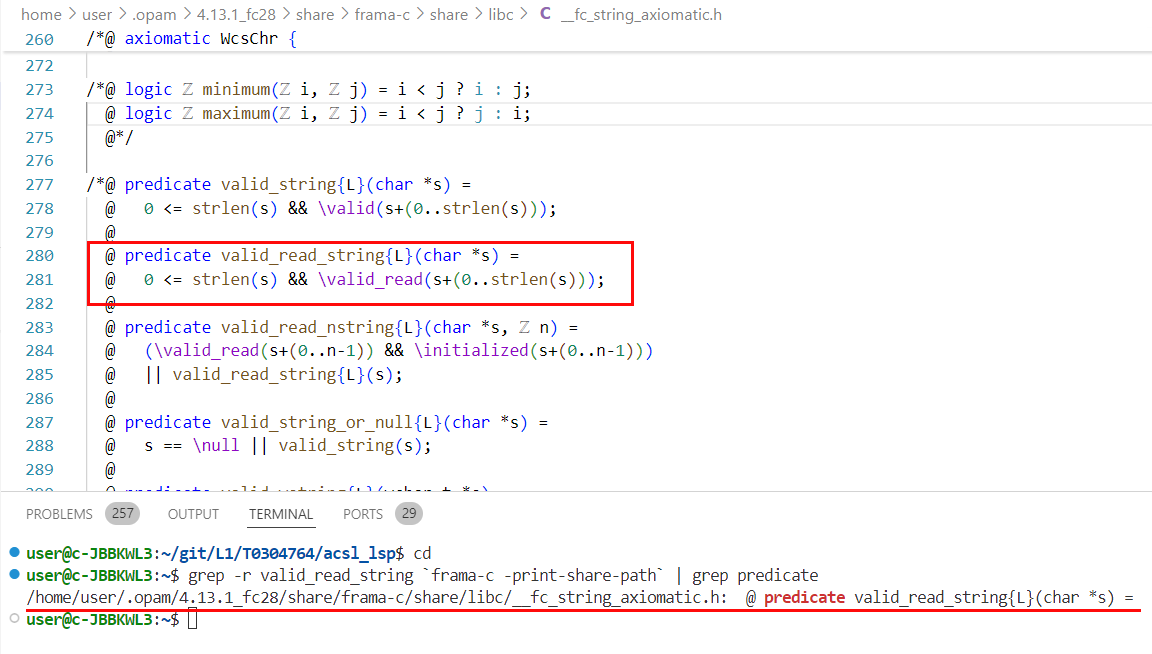
\includegraphics[scale=0.7]{grep.png}
	\caption{Example of searching predicate definition with grep}
\end{figure}

Searching through potentially large directories and files using grep is time-consuming, especially when dealing with complex libraries with numerous functions and predicates.
This method relies heavily on manual effort and familiarity with command-line tools, which can be error-prone and inconvenient.

The inefficiencies of the current method emphasize the necessity for a more streamlined solution. A Language Server Protocol (LSP) tailored for ACSL code would offer significant improvements by providing features such as real-time code browsing, automatic function and predicate lookup, contextual information, and integration with the editing environment. Such a tool would greatly enhance productivity by automating these tasks and reducing the reliance on cumbersome manual search processes.

Additionally, those unaccustomed to Frama-C and ACSL annotations can benefit from this solution for getting started and have a better understanding of the specification language.

The goal of this project is to develop a software solution to offer language programming features for C/ACSL in IDEs including code navigation, completion suggestions, and interaction with Frama-C code analysis, to enhance validation and facilitate certification at EAL6/EAL7 levels of the Common Criteria.


\subsection{Work organization}
% TODO : mettre le project plan sous forme d'histogramme


\section{Background}
\subsection{The Language Server Protocol}
\subsubsection{Introduction}
Developers working on large scale projects often need a code editing environment with the adequate tooling for the languages they use in their workspace. Multiple solutions such as Eclipse or IntelliJ IDEA exist for Java projects, as well as other popular programming languages. But the complexity of developing one tool for one language and one specific editor is tedious as it forces developers to implement the same language programming features for every code editor with each programming language. To overcome these, a solution was developed: the Language Server Protocol (LSP)\footnote{https://microsoft.github.io/language-server-protocol/overviews/lsp/overview/}.

The language Server Protocol (LSP) is built on top of the \href{https://www.jsonrpc.org/specification}{JSON-RPC protocol}, a remote procedure call protocol that uses JSON as data format.
It permits a communication between a client and a server.

The Language Server Protocol (LSP) operates through a structured communication system between the client (such as an IDE or code editor) and the server (which provides language-specific features). This communication is facilitated by various types of messages and methods that define the interactions between the client and server.

Request Message: A request message is sent by the client to ask the server to perform a specific action. Each request is associated with a particular method, which determines the type of operation being requested. For example, methods like `textDocument/completion' request code completion suggestions, while `textDocument/definition' asks for the location of a symbol's definition. These requests expect a response from the server, which will either provide the requested data or indicate an error.

Notification Message: Notification messages are used by the client to inform the server of events or changes in the editor, such as opening, modifying, or closing a document. Unlike request messages, notifications do not expect a response. They keep the server updated on the current state of the workspace. Methods associated with notifications include `textDocument/didOpen', `textDocument/didChange', and `textDocument/didClose'.


\paragraph*{LSP features Organization} 



\begin{figure}[H]
	\centering
	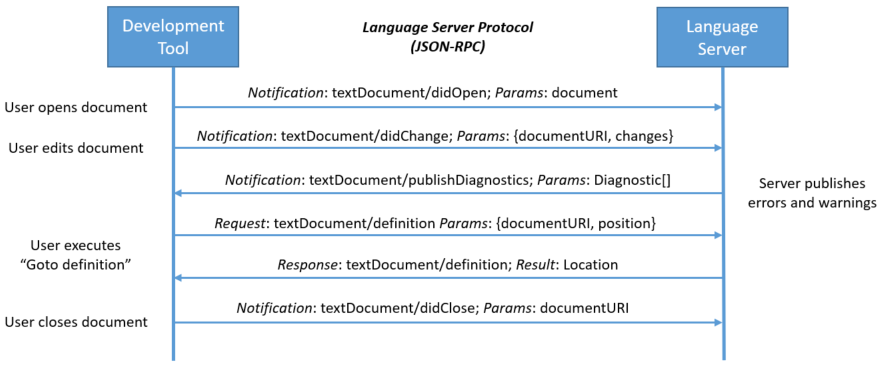
\includegraphics[scale=0.4]{lsp_exchange_example.png}
	\caption{Language Server Protocol sequence diagram: example of an interaction flow between client and server}
\end{figure}

\subsubsection{LSP Capabilities}
The LSP defines sets of features named `capabilities'. LSP capabilities are boolean values transported in a JSON request that each party declares when the extension is launched.
These declarations are needed so that both agree on which features each can provide. Only the features supported by both parties can be used in the editor. 

Capabalities can be registered in two ways: statically and dynamically.
Static registration is done through the initialize request, so it is done once and for all.
Dynamic registration allows language servers to add or remove support for various capabilities at runtime without a reinitialization of the server. 

Below is a sequence diagram of the first requests exchanged between the client and the server, the user can start using the extension once the server has received the `initialized' notification by the the client (not to be confused with the `initialize' request)
\begin{figure}[H]
	\centering
	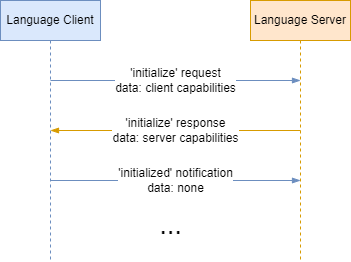
\includegraphics[scale=0.7]{diag2.drawio.png}
	\caption{Sequence diagram of the `initialize' request}
\end{figure}

\subsubsection{Features}

LSP features are organized into categories based on the type of operations they perform. These categories include:

Text Document Features: These features deal with operations on text documents, such as opening, editing, saving, and closing files. Examples include `textDocument/didOpen', `textDocument/didChange', and `textDocument/didSave`.

Language Features: These features provide language-specific features such as autocompletion, go-to-definition, hover information, and find-references. Examples include `textDocument/completion', `textDocument/definition', and `textDocument/hover'.

Workspace Features: These features relate to operations that affect the entire workspace, such as searching for symbols or managing project settings. Examples include `workspace/symbol' and `workspace/configuration'.

\textcolor{red}{TODO : example of features and example of corresponding json for each feature, ref to the appendix for full listing of lsp features}
\begin{longtable}
    \begin{tabular}{|l|l|}
		\hline
		\textbf{Feature} &
		\textbf{JSON} \\ \hline
		Definition 					& 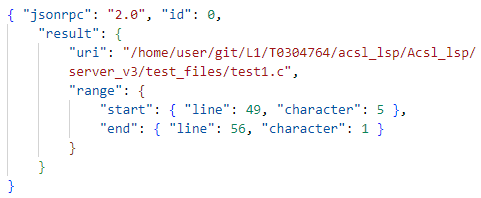
\includegraphics[scale=0.7]{definition_result.png} \\ \hline
		Declaration 				& 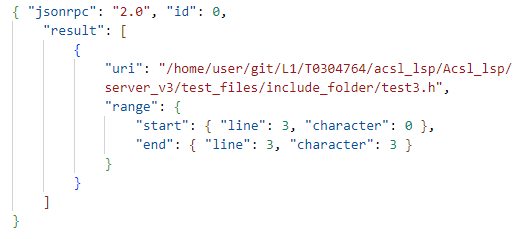
\includegraphics[scale=0.7]{declaration_result.png} \\ \hline
		Display CIL 				& 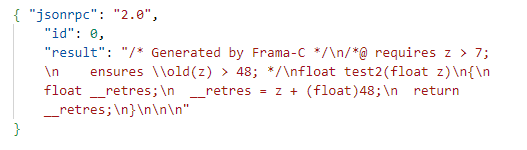
\includegraphics[scale=0.7]{display_cil_result.png} \\ \hline
		Callgraph 					& 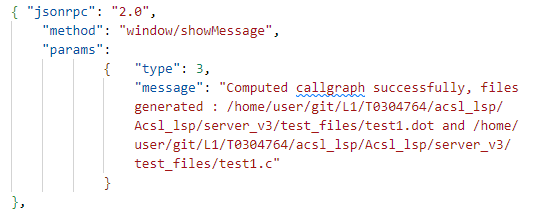
\includegraphics[scale=0.7]{callgraph_result.png} \\ \hline
		Local Metrics 				& 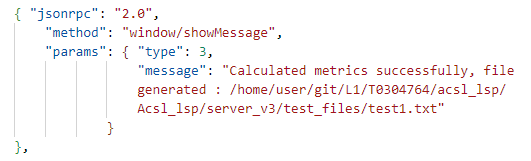
\includegraphics[scale=0.7]{local_metrics_result.png} \\ \hline
		Global Metrics 				& 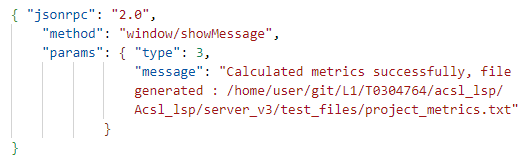
\includegraphics[scale=0.7]{global_metrics_result.png} \\ \hline
		Proof Obligations 			& 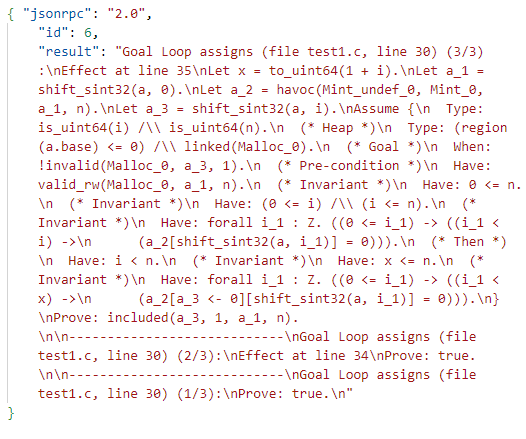
\includegraphics[scale=0.7]{po_result.png} \\ \hline
		Prove Annotation 			& Not implemented \\ \hline
		Diagnostics 				& -metrics, -metrics-output \\ \hline
    \end{tabular}
	\caption{Example of corresponding JSON for each feature}
    \label{tab:features-json}
\end{longtable}

\begin{table}
	\centering
    \caption{Option details}
    \label{tab:features-options-details}
    \begin{tabular}{|l|l|l|l|p{0.2cm}|p{0.2cm}|p{0.2cm}|p{0.2cm}|p{0.2cm}|p{0.2cm}|p{0.2cm}|p{0.2cm}|}
    \hline
    \textbf{Client option} &
      \rot{\textbf{Advanced}} &
      \rot{\textbf{Definition}} &
      \rot{\textbf{Declaration}} &
      \rot{\textbf{Display CIL}} &
      \rot{\textbf{Callgraph}} &
      \rot{\textbf{Local Metrics}} &
      \rot{\textbf{Global Metrics}} &
      \rot{\textbf{Proof Obligations}} &
      \rot{\textbf{Prove Annotation}} &
      \rot{\textbf{Diagnostics}} \\ \hline
    acslLsp							&   & X & X & X & X & X & X & X & X & X \\ \hline
    kernel.sourceFiles						&   & X & X &   &   &   & X &   &   & X \\ \hline
    kernel.includePaths  					&   & X & X & X & X & X & X & X & X & X \\ \hline
    kernel.macros							&   & X & X & X & X & X & X & X & X & X \\ \hline
    kernel.machdep 						&   &   &   & X & X & X & X & X & X & X \\ \hline
    kernel.keepUnusedSpecifiedFunctions 	&   & X & X & X & X & X & X & X & X & \\ \hline
    kernel.aggressiveMerging			 	&   & X & X & X & X & X & X & X & X &  \\ \hline
    kernel.generatedSpecCustom 			& Yes &   &   & X & X & X & X & X &   &   \\ \hline
    metrics.output 					&   &   &   &   & X & X & X &   &   & \\ \hline
	callgraph.output						&   &   &   &   & X &   &   &   &   & \\ \hline
    callgraph.roots							&   &   &   &   & X &   &   &   &   & \\ \hline
    callgraph.services 					&   &   &   &   & X &   &   &   &   & \\ \hline
    wp.rte 							&   &   &   &   &   &   &   &   & X &   \\ \hline
    wp.checkMemoryModel 				& Yes &   &   &   &   &   &   &   & X &   \\ \hline
    wp.volatile 						& Yes &   &   &   &   &   &   &   & X &   \\ \hline
    wp.pruning 					& Yes &   &   &   &   &   &   &   & X &   \\ \hline
    wp.prover 						&   &   &   &   &   &   &   &   & X &   \\ \hline
    wp.timeout 						&   &   &   &   &   &   &   &   & X &   \\ \hline
    wp.session 						&   &   &   &   &   &   &   &   & X &   \\ \hline
	diagnostics.wp 					&   &   &   &   &   &   &   &   &   & X \\ \hline
    \end{tabular}
\end{table}

\subsection{Frama-C plugin development}
\textcolor{red}{describe working example, comment on crée un plugin, dune (librairies, entry point)}

\textcolor{red}{describe the kernel api, wp api and modules that are relevant to implement the LSP}

\textcolor{red}{parler de l'invariant : un seul ast par projet}
Frama-C is an extensible platform for the static analysis of C programs. Its architecture allows for the development of custom plugins, which can leverage the existing infrastructure and libraries provided by Frama-C to perform specialized analyses. This section provides an overview of the process and tools available for developing a Frama-C plugin, focusing on the key libraries, modules, and APIs that support plugin development.

\subsubsection{Frama-C Architecture Overview}
The Frama-C framework is composed of several core components that facilitate the development of plugins:

\paragraph*{Kernel Library}{The Kernel is the backbone of Frama-C, responsible for managing the project lifecycle, abstract syntax trees (AST), and the overall data flow within the platform. It provides essential services such as parsing C source files, type checking, and maintaining the internal representation of the program being analyzed.}

\paragraph*{Control Flow Graph (CFG)}{The CFG plug-in is central to performing control flow analysis in Frama-C. It allows the construction and manipulation of control flow graphs, which represent all possible paths of execution in a program. Plugins that need to analyze or transform the control flow of a program rely heavily on this module.}

\paragraph*{Deductive Verification (WP)}{The WP plugin is used to generate verification conditions using the weakest precondition calculus. These conditions are then checked to ensure that the program adheres to its formal specification, typically expressed in ACSL (ANSI/ISO C Specification Language). This module is crucial for plugins aimed at formal verification or proof-based analysis.}

\paragraph*{Metrics}{This module computes various code metrics, such as cyclomatic complexity and lines of code. These metrics are often used to assess the quality and maintainability of the code, making this module useful for plugins focused on code quality analysis.}

\subsubsection{Steps in Developing a Plugin}
Developing a plugin for Frama-C involves several methodical steps, each crucial for ensuring that the plugin integrates seamlessly with the existing Frama-C infrastructure:

\textbf{Environment Setup}: Plugin development in Frama-C requires proficiency in OCaml, as both Frama-C and its plugins are implemented in this language. Developers must set up an OCaml development environment and obtain the Frama-C source code along with its dependencies.

\textbf{Plugin Initialization}: The development of a Frama-C plugin begins with defining the plugin module in OCaml. This involves registering the plugin with the Frama-C Kernel, specifying metadata such as the plugin’s name, version, and a brief description.

\textbf{Interfacing with the Kernel}: Once the plugin is initialized, it must interface with the Frama-C Kernel to access the AST, CFG, or other program representations. The Kernel API provides various functions to manipulate these representations, allowing the plugin to register callbacks or hooks during specific analysis phases.

\textbf{Utilizing Core Modules}: Depending on the analysis goals, the plugin may need to interact with specific Frama-C modules like CFG or WP. For instance, a plugin designed to analyze the control flow of a program will use the CFG module to traverse and manipulate the CFG.

\textbf{Testing and Debugging}: During the development process, it is essential to test and debug the plugin thoroughly. Frama-C offers logging and debugging facilities that allow developers to track the plugin's execution and identify potential issues.

\textbf{Command-Line Integration}: After implementing the core functionality, the plugin needs to be integrated with Frama-C’s command-line interface (CLI). This integration enables users to invoke the plugin directly from Frama-C, using standard command-line options.

\textbf{Documentation and User Support}: Frama-C encourages developers to document their plugins thoroughly. This includes embedding help messages within the plugin and providing external documentation to assist users in understanding the plugin’s functionality and usage.

\subsubsection{Supporting Tools and Resources for Plugin Development}
Frama-C offers a comprehensive set of tools and resources to assist developers in creating high-quality plugins:

\textbf{API Documentation}: The Frama-C API provides an online API where we can browse each plug-in's library and better understand its functions.

\textbf{Plugin Guide}: Frama-C provides a tutorial for developing a new plugin, serving as a starting point that includes basic setup and interaction with the Frama-C Kernel library.

\textbf{Community Support}: Frama-C community provides mailing lists and forums for plugin developers.

\subsection{VS Code Extensions}

\textcolor{red}{working example (extension plaintext), comment est organisé une extension typescript}

The architecture of VS Code extensions is based on a client-server model, which aligns perfectly with the Language Server Protocol. VS Code provides an API with TypeScript libraries for developing different types of extensions, particularly, language extensions. 
A language extension offers declarative (e.g.\: syntax highlighting, bracket autoclosing) and programmatic (e.g.\: hover information, jump to definition) language features. 

\subsubsection{ACSL extensions}
Very few VS Code extensions for Frama-C exist in the marketplace\footnote{The Visual Studio marketplace where VS Code extension can be installed}.
The only extensions related to Frama-C are for ACSL syntax coloration made by an independent developer\footnote{https://github.com/MisterZurg}. 

The first one, `ACSL-lite'\footnote{https://github.com/MisterZurg/acsl-lite} removes syntax coloration for C code and adds coloration for ACSL annotations, but it has no other feature. The drawback of this extension is that it removes entirely the coloration for C when we also need it. 

The second one `ACSL:\@ ANSI/ISO C Specification Language'\footnote{https://github.com/MisterZurg/acsl-ansi-iso-c-specification-language} has coloration for both ACSL and C. But there are a few fixes to make.

\subsubsection{VS Code IntelliSense}


\section{Design Choices}
\subsection{Server}
The server was implemented as a Frama-C plug-in to fully exploit the advanced parsing and analysis capabilities inherent in the Frama-C framework. Frama-C is a powerful platform for source code analysis of C programs, offering a wide range of tools and libraries tailored for static analysis. By developing the server as a plug-in within this ecosystem, we can directly leverage these pre-existing tools.

The server itself is an OCaml application that facilitates communication between the Frama-C plug-in and external clients. This design choice allows us to maintain a modular architecture where the core analysis logic remains within the Frama-C environment, ensuring that it benefits from continuous updates and improvements made to the Frama-C platform. The server acts as an intermediary, managing interactions between the Frama-C plug-in and the client, which can be an independent application requiring code analysis services. 

This architecture---comprising the server executable, the Frama-C plug-in, and the client---ensures a clear separation of concerns. The server handles communication and orchestration, the plug-in performs the specialized analysis tasks, and the client interfaces with the server to request these services. This modularity not only enhances maintainability but also allows for flexibility in extending or adapting any of the components as needed.

\subsection{Communication}
Unix sockets were selected as the communication mechanism among the three components---server, Frama-C plug-in, and client---due to their efficiency and simplicity in local inter-process communication (IPC). Unlike other IPC methods such as pipes or shared memory, Unix sockets provide a versatile and robust means of exchanging data between processes running on the same machine.

The decision to use Unix sockets over other alternatives like TCP/IP sockets was driven by the need for low-latency and secure communication in a local environment. Since the processes are all located on the same host, Unix sockets offer a significant performance advantage by avoiding the costs associated with network protocol layers, which are unnecessary in this context.

Furthermore, the OCaml Unix module, which provides native support for Unix sockets, allows ideal integration with the existing OCaml-based infrastructure of the server. This compatibility ensures that data is transmitted efficiently. By leveraging Unix sockets, we achieve a communication mechanism that is not only fast and reliable but also well-suited to the architecture of the application.

\textcolor{red}{parler du handler (1 command par feature)}

\textcolor{red}{algo du handler}

\subsection{Architecture}


\textcolor{red}{vscode = serveur}
\textcolor{red}{TODO : options de notre plugin, celles qui peuvent pas s'activer en meme temps,}

\textcolor{brown}{
	The first purpose of this project is to implement a language server for ACSL/C, so the project will forcibly have a directory with the server code in it.
	But we also want a client that will use it and we chose vs code. Now we have a default client, so there is a need for a directory with the source code of the client.
	We decided to put the client in the same project as the server so when the user installs it it comes as a bundle, instead of letting the user install them separately, since the source code of the vs code client consists of only file.
	As said earlier, in theory, the server should work with any client, but we have not tested with other clients, and we do not know how the other clients handle the server process: for example, vs code creates the process and the frama-c plug-in connects to it, but do not know if other plug-ins function the same way. So all features and issues encountered during this internship, concern the combination of the Frama-C plug-in with the VS Code extension. In this report, we will refer to the plug-in directly as the server to avoid confusion.
	We chose the architecture of our project as follows: we create one OCaml module per feature, (e.g.: `Go To Definition' feature will be handled by a module written in file `definition.ml').
}


\subsection{A first approach on the server implementation}
In the context of Frama-C, an execution instance, whether initiated via the command line or through a function call within the Frama-C library, is referred to as a session. Initially, we considered implementing the server directly as a Frama-C plug-in, where the main loop responsible for handling Language Server Protocol (LSP) requests would be executed within this plug-in. This approach would handle all LSP requests into a single, continuous session.

However, this design presented a significant drawback: when Frama-C encounters a syntax error during file parsing, the entire session enters an error state. Given that a session in this context would persist until the server either crashes or the client terminates it, the error state would persist indefinitely. This is problematic because even if the user corrects the error in the code, the session---and consequently the server---would remain in the error state.

Terminating the session as a response to an error is not a viable solution, as it would lead to the server's shutdown. This, in turn, would cause the client to disconnect, leading to a crash of the extension. Consequently, the user would need to manually restart the extension, which is an undesirable outcome. To avoid such disruptions and maintain a seamless user experience, it is imperative that the server architecture be designed to handle errors more gracefully without necessitating a session termination.

\subsection{plug-in installation}
% TODO : 
% - choix de la methode de communication : sockets OK
% - choix du serveur en tant que plug-in frama-c OK
% - choix du langage ocaml 
% - parler de la premiere approche avec le plug-in qui contient la boucle principale directement puis expliquer pourquoi cette solution ne marchait pas
% - choix de l'architecture du plug-in


% - ajouter une sous section pour les features et les détailler, parler des fonctionnalités non LSP, fonctionnailté VS Code (colo syntaxique)

\section{Development}

\textcolor{red}{ TODO : working example (extension plaintext ?), comment est organisé une extension typescript}
\subsection{TypeScript extension organization}
The outline of the client code is presented as follows :
\begin{itemize}
	\item .eslintignore: The .eslintignore file is used to specify patterns that should be ignored by ESLint, a popular JavaScript linter. ESLint is a tool that analyzes JavaScript code for potential errors, and other issues.
	\item .eslintrc.js: allows us to tailor ESLint's behavior to align with our project's coding standards and requirements
	\item .vscode:  holds configuration files that customize the behavior of Visual Studio Code for the project, e.g.: how the extension is launched via launch.json
	\item README.md: contains description and installing instructions about the client
	\item language-configuration.json: controls the following Declarative Language Features: Comment toggling, Brackets definition, Autoclosing, Autosurrounding, Folding Word pattern, Indentation Rules ...
	\item node\_modules: Javascript/Typescript dependencies used in the project, generated with `npm install'
	\item out: Javascript executable files generated from typescript source code by `npm run compile'
	\item package-lock.json: file generated from package.json when running `npm install'
	\item package.json: VS Code extension package configuration, contains description, information about installed dependencies and scripts to build the project
	\item scripts: contains end-to-end testing shell script 
	\item src: contains typescript source code that launches the language client
	\item syntaxes: contains TextMate language grammar for syntax coloration
	\item tsconfig.json: configure the behavior of the TypeScript compiler (tsc)
\end{itemize}


\subsection{Working example}


\subsection{Project configurations}

\textcolor{green}{tableau feature/parsing local (.h ou .c) ou global (spécifié par user ou par defaut que les fichiers .c)}

\textcolor{magenta}{tableau de chaque feature et sa ligne de commande frama-c (usage de -then et -then-last) faire le lien avec les configs}

\textcolor{green}{listing de toutes les options, leur organisation}
\begin{table}
	\centering
    \caption{Frama-C options available to the user}
    \label{tab:features-options}
    \begin{tabular}{|l|l|l|}
		\hline
		\textbf{Client option} &
		\textbf{Plug-in} &
		\textbf{Frama-C option(s)} \\ \hline
		acslLsp 						& ACSL LSP    & -lsp-debug	\\ \hline
		kernel.includePaths 					& Kernel    & -cpp-extra-args \\ \hline
		kernel.macros 							& Kernel    & -cpp-extra-args \\ \hline
		kernel.sourceFiles 					& Kernel    &  \\ \hline
		kernel.machdep 						& Kernel    & -machdep \\ \hline
		kernel.keepUnusedSpecifiedFunctions 	& Kernel    & -remove-unused-specified-functions \\ \hline
		kernel.aggressiveMerging 				& Kernel    & -aggressive-merging \\ \hline
		kernel.generatedSpecCustom 			& Kernel    & -generated-spec-custom \\ \hline
		metrics.output 					& Metrics   & -metrics, -metrics-output \\ \hline
		callgraph.output 							& Callgraph & -cg, -cg-roots \\ \hline
		callgraph.roots 							& Callgraph & -cg, -cg-roots \\ \hline
		callgraph.services 					& Callgraph & -cg, -cg-no-services \\ \hline
		wp.rte 							& WP & -wp, -wp-rte \\ \hline
		wp.checkMemoryModel 			& WP & -wp, -wp-check-memory-model \\ \hline
		wp.volatile 					& WP & -wp, -wp-volatile \\ \hline
		wp.noPruning 					& WP & -wp, -wp-no-pruning \\ \hline
		wp.prover 						& WP & -wp, -wp-prover \\ \hline
		wp.timeout 						& WP & -wp, -wp-timeout \\ \hline
		wp.session 						& WP & -wp, -wp-session \\ \hline
		diagnostics.wp 					& ACSL LSP & -lsp-wp \\ \hline
    \end{tabular}
\end{table}



\textcolor{green}{tableau feature/module api frama-c utilisé}
\textcolor{red}{tableau algo principal de chaque feature}
\textcolor{red}{tableau des capacités du serveur}


\subsection{`Go To Definition' feature}
The `Go To Definition' feature of Visual Studio Code allows developers to easily navigate to the definition of symbols within their code. In this context, the challenges involve implementing a VS Code extension that supports this feature for two languages associated with the same file extension (`.c' and `.h'). 

When a user requests to find the definition of a symbol at a specific position in the code, the server first identifies the name of the symbol located at that position. This involves parsing, analyzing the file and extracting the relevant word based on the provided line and column numbers.
The code then initiates a search through various subsections of the code to find where the symbol is defined. This search involves visiting different parts of the source file's Abstract Syntax Tree (AST) and concerns both ACSL and C code:
\begin{itemize}
\item ACSL Definitions: The code checks if the symbol matches any logical predicates or terms, which are specific to tools like Frama-C used for static analysis of C programs.
\item C Definitions: It examines global entities, such as enums, structures, functions, and variables, to see if the symbol matches any of these.
\end{itemize}
Each of these searches uses visitor patterns, which traverse and inspect nodes in the AST, comparing each node's name to the symbol's name.

If a definition is located, the exact file path and the range of lines and columns where the symbol is defined are packaged into a JSON response. If no definition is found, a response indicating a null result is returned. This response allows the LSP client (the user's text editor or IDE) to navigate directly to the symbol's definition or handle the case where no definition exists.


\subsection{File Synchronization \& Diagnostics}
File synchronization is a key feature of the LSP\@. Three types of requests are sent by VS Code to notify document opening, changing and saving actions performed by the user. 
A single file parsing is performed each time a file is opened or saved. We add an event listener to catch any error or warning raised by the Frama-C parser and we store them inside a JSON block.
All diagnostics are published to the editor and displayed to the user in the form of squiggles and listed in the `Problems' subsection of the VS Code terminal/console (?).

There are two types of diagnostics: warnings and errors. Warnings are raised in case an ACSL annotation is not formed properly or when an unknown function is called. Errors are raised when there is a syntax error in the C code preventing the parser to finish (which are fatal errors). In the latter case, normally, any Frama-C session stops, but we ensure that diagnostics are sent either in case the parsing succeeds or fails. So we send them just before the exception aborts fatally.
In case the parsing succeeds without any messages, the diagnostics are cleared in the editor.

The listener is a Frama-C function that reports any event emitted by Frama-C while parsing. From those events we can extract their source, their message and their kind (whether it is an error, a warning a feedback, etc.). By manipulating these data, we organize them and adapt them to the LSP standard.

This feature is only implemented for single file parsing and diagnostics are computed only when the file is saved. No diagnostics are published for multiple file parsing, which means we do not know if those files are in state of error. So the user has to make sure the source files they provided have no errors.

\subsection{File parsing}
In order to use the Frama-C module's functions, the plug-in converts the source code files into their C Intermediate Language (CIL) representation, which provides a detailed hierarchical structure of the source code. It captures the syntactic elements and relationships within the code, for deeper analysis and processing. This representation allows the server to efficiently navigate and manipulate the code, supporting features like `Go To Definition' and other code navigation tools.

The system is designed to handle the parsing of both single and multiple source code files. Regardless of the number of files being parsed, the resulting Abstract Syntax Trees (ASTs) from each file are merged into a single one. This merging process is crucial as it simplifies the analysis and manipulation of the code, providing a unified structure that the server can work with more effectively.

When dealing with large codebases, users often face the challenge of working with a vast number of source files. Parsing all these files can be a time-consuming task. To address this issue, the system offers a Visual Studio Code setting that allows users to specify which source files need to be parsed. By focusing the parsing process on only the relevant files, this setting helps optimizing the time spent on parsing, making the workflow more efficient.

Users must ensure that all necessary source files are included in the parsing process. If a user fails to specify a source file that is needed for certain features, such as Go To Definition, they may not function correctly. It is therefore the responsibility of the user to provide all the relevant files.


\section{LSP use cases with VS Code}
% TODO : mettre en annexe les tableaux
In this enclosed figure is a listing of all LSP features, if they are handled by VS Code, and their implementation status on the server side.
\begin{table}[]
	\centering
	\caption{Features implementation details}
	\label{tab:features-implementation-details}
	\begin{tabular}{|p{1in}|p{2in}|l|l|}
	\hline
	\textbf{Feature}                             & \textbf{Related Frama-C API modules}        & \textbf{Main algorithm} & \textbf{Parsing mode} \\ \hline
	Go To Declaration   & Cil, Visitor, Filepath, File, Ast, Json & Tree traversal & Global \\ \hline
	Go To Definition    & Cil, Visitor, Filepath, File, Ast, Json & Tree traversal & Global \\ \hline
	Diagnostics         & Filepath, File, Log, Json               & Event listener & Local  \\ \hline
	Display CIL of file & Ast, Printer, Pretty\_utils, Json       & Get            & Local  \\ \hline
	Show proof obligations of annotation(s)/file & WP, Property, Filepath, Json, Pretty\_utils & List traversal          & Local                 \\ \hline
	Show proof verdict  &                                         & List traversal & Local  \\ \hline
	Compute Callgraph   & Callgraph                               & Get            & Local  \\ \hline
	Show Metrics        & Metrics                                 & Get            & Local  \\ \hline
	\end{tabular}
\end{table}

\begin{longtable}{|p{2in}|p{3in}|l|l|}
	\hline
	\multicolumn{1}{|l|}{\textbf{LSP features}} &
	  \multicolumn{1}{l|}{\textbf{Use case(s)}} &
	  \multicolumn{1}{l|}{\textbf{Implementation status}} &
	  \textbf{Supported by VS Code} \\ \hline
	\multicolumn{4}{|l|}{Language features} \\ \hline
	\multicolumn{1}{|l|}{Go to Declaration} &
	  \multicolumn{1}{l|}{Show declaration of C library, Frama-C and user defined functions, variables, macros, types, ACSL types, ACSL terms and predicates.} &
	  \multicolumn{1}{l|}{Implemented} &
	  Yes \\ \hline
	\multicolumn{1}{|l|}{Go to Definition} &
	  \multicolumn{1}{l|}{Show definition of C library, Frama-C and user defined functions, variables, macros, types, ACSL types, ACSL terms and predicates.} &
	  \multicolumn{1}{l|}{Implemented} &
	  Yes \\ \hline
	\multicolumn{1}{|l|}{Go to Type Definition} &
	  \multicolumn{1}{l|}{Show definition of C library, Frama-C and user defined functions types} &
	  \multicolumn{1}{l|}{Implemented (included in go to definition)} &
	  Yes \\ \hline
	\multicolumn{1}{|l|}{Go to Implementation} &
	  \multicolumn{1}{l|}{Show implementation of C library, Frama-C and user defined functions, variables, macros, types, ACSL types, ACSL terms and predicates.} &
	  \multicolumn{1}{l|}{} &
	  Yes \\ \hline
	\multicolumn{1}{|l|}{Find References} &
	  \multicolumn{1}{l|}{Show references of C library, Frama-C and user defined functions, variables, macros, types, ACSL types, ACSL terms and predicates.} &
	  \multicolumn{1}{l|}{} &
	  Yes \\ \hline
	\multicolumn{1}{|l|}{Prepare Call Hierarchy} &
	  \multicolumn{1}{l|}{Prepare call hierarchy of C functions, ACSL terms and predicates} &
	  \multicolumn{1}{l|}{} &
	  Yes \\ \hline
	\multicolumn{1}{|l|}{Call Hierarchy Incoming Calls} &
	  \multicolumn{1}{l|}{List incoming calls of C functions} &
	  \multicolumn{1}{l|}{} &
	  Yes \\ \hline
	\multicolumn{1}{|l|}{Call Hierarchy Outgoing Calls} &
	  \multicolumn{1}{l|}{List outgoing calls of C functions} &
	  \multicolumn{1}{l|}{} &
	  Yes \\ \hline
	\multicolumn{1}{|l|}{Prepare Type Hierarchy} &
	  \multicolumn{1}{l|}{Prepare type hierarchy of C types} &
	  \multicolumn{1}{l|}{} &
	  Yes \\ \hline
	\multicolumn{1}{|l|}{Type Hierarchy Super Types} &
	  \multicolumn{1}{l|}{List super types of C types} &
	  \multicolumn{1}{l|}{} &
	  Yes \\ \hline
	\multicolumn{1}{|l|}{Type Hierarchy Sub Types} &
	  \multicolumn{1}{l|}{List sub types of C types} &
	  \multicolumn{1}{l|}{} &
	  Yes \\ \hline
	\multicolumn{1}{|l|}{Document Highlight} &
	  \multicolumn{1}{l|}{Highlight occurrences of all words OR only C library, Frama-C and user defined functions, variables, macros, types, ACSL types, ACSL terms and predicates} &
	  \multicolumn{1}{l|}{} &
	  Yes \\ \hline
	\multicolumn{1}{|l|}{Document Link} &
	  \multicolumn{1}{l|}{Shows links written inside C and ACSL comments and make them browsable} &
	  \multicolumn{1}{l|}{} &
	  Yes \\ \hline
	\multicolumn{1}{|l|}{Document Link Resolve} &
	  \multicolumn{1}{l|}{Related to Document Link} &
	  \multicolumn{1}{l|}{} &
	  Yes \\ \hline
	\multicolumn{1}{|l|}{Hover} &
	  \multicolumn{1}{l|}{Show C function contract, show C function type information and documentation if available} &
	  \multicolumn{1}{l|}{} &
	  Yes \\ \hline
	\multicolumn{1}{|l|}{Code Lens} &
	  \multicolumn{1}{l|}{Show C function signature} &
	  \multicolumn{1}{l|}{} &
	  Yes \\ \hline
	\multicolumn{1}{|l|}{Code Lens Refresh} &
	  \multicolumn{1}{l|}{Refresh C function signature if changes were made} &
	  \multicolumn{1}{l|}{} &
	  Yes \\ \hline
	\multicolumn{1}{|l|}{Folding Range} &
	  \multicolumn{1}{l|}{Fold function contracts, functions, function descriptions, comments, ghost code} &
	  \multicolumn{1}{l|}{} &
	  Yes \\ \hline
	\multicolumn{1}{|l|}{Selection Range} &
	  \multicolumn{1}{l|}{Suggest selection range of function contracts, functions, function descriptions, comments, ghost code} &
	  \multicolumn{1}{l|}{} &
	  Yes \\ \hline
	\multicolumn{1}{|l|}{Document Symbols} &
	  \multicolumn{1}{l|}{List (in the current file) symbols of C functions, variables, ACSL terms and predicates.} &
	  \multicolumn{1}{l|}{} &
	  Yes \\ \hline
	\multicolumn{1}{|l|}{Semantic Tokens} &
	  \multicolumn{1}{l|}{Request semantic tokens for C and ACSL keywords to provide additional color information.} &
	  \multicolumn{1}{l|}{} &
	  Yes \\ \hline
	\multicolumn{1}{|l|}{Inline Value} &
	  \multicolumn{1}{l|}{Show, at the end of the line, the values of C variables in a line} &
	  \multicolumn{1}{l|}{} &
	  Yes \\ \hline
	\multicolumn{1}{|l|}{Inline Value Refresh} &
	  \multicolumn{1}{l|}{Refresh the values of C variables in a line if changed} &
	  \multicolumn{1}{l|}{} &
	  Yes \\ \hline
	\multicolumn{1}{|l|}{Inlay Hint} &
	  \multicolumn{1}{l|}{No use cases found} &
	  \multicolumn{1}{l|}{} &
	  Yes \\ \hline
	\multicolumn{1}{|l|}{Inlay Hint Resolve} &
	  \multicolumn{1}{l|}{No use cases found} &
	  \multicolumn{1}{l|}{} &
	  Yes \\ \hline
	\multicolumn{1}{|l|}{Inlay Hint Refresh} &
	  \multicolumn{1}{l|}{No use cases found} &
	  \multicolumn{1}{l|}{} &
	  Yes \\ \hline
	\multicolumn{1}{|l|}{Moniker} &
	  \multicolumn{1}{l|}{No uses cases found} &
	  \multicolumn{1}{l|}{} &
	  Yes \\ \hline
	\multicolumn{1}{|l|}{Completion Proposals} &
	  \multicolumn{1}{l|}{\begin{tabular}[c]{@{}l@{}}Show completion item for ACSL : ACSL keywords completion (ensures, assigns, etc.)\\ - propose variables bound to the current file or workspace\\ - C keyword completion.\end{tabular}} &
	  \multicolumn{1}{l|}{Ongoing but disabled} &
	  Yes \\ \hline
	\multicolumn{1}{|l|}{Completion Item Resolve} &
	  \multicolumn{1}{l|}{Extend Completion Proposals feature} &
	  \multicolumn{1}{l|}{} &
	  Yes \\ \hline
	\multicolumn{1}{|l|}{Publish Diagnostics} &
	  \multicolumn{1}{l|}{Show compilation errors, warnings for C and ACSL code.} &
	  \multicolumn{1}{l|}{} &
	  Yes \\ \hline
	\multicolumn{1}{|l|}{Pull Diagnostics} &
	  \multicolumn{1}{l|}{Related to Publish Diagnostics} &
	  \multicolumn{1}{l|}{} &
	  Yes \\ \hline
	\multicolumn{1}{|l|}{Signature Help} &
	  \multicolumn{1}{l|}{Show C library, Frama-C and user defined function signatures when function name is typed} &
	  \multicolumn{1}{l|}{} &
	  Yes \\ \hline
	\multicolumn{1}{|l|}{Code Action} &
	  \multicolumn{1}{l|}{The server can provide code actions related to a diagnostic such as fixing includes, etc.} &
	  \multicolumn{1}{l|}{} &
	  Yes \\ \hline
	\multicolumn{1}{|l|}{Code Action Resolve} &
	  \multicolumn{1}{l|}{Related to Code Action} &
	  \multicolumn{1}{l|}{} &
	  Yes \\ \hline
	\multicolumn{1}{|l|}{Document Color} &
	  \multicolumn{1}{l|}{Show color of ANSI color codes in the C code if any (when printing colors in the terminal, etc.)} &
	  \multicolumn{1}{l|}{} &
	  Yes \\ \hline
	\multicolumn{1}{|l|}{Color Presentation} &
	  \multicolumn{1}{l|}{Related to Document Color} &
	  \multicolumn{1}{l|}{} &
	  Yes \\ \hline
	\multicolumn{1}{|l|}{Formatting} &
	  \multicolumn{1}{l|}{Fix indentations in C file for C and ACSL code.  Provide indentation levels for ACSL code. Carriage return after each semi-colon, spaces between symbols, arithmetic and logic operators.} &
	  \multicolumn{1}{l|}{} &
	  Yes \\ \hline
	\multicolumn{1}{|l|}{Range Formatting} &
	  \multicolumn{1}{l|}{Fix indentations in C file for C and ACSL code.  Provide indentation levels for ACSL code. Carriage return after each semi-colon, spaces between symbols, arithmetic and logic operators for selected lines in the code.} &
	  \multicolumn{1}{l|}{} &
	  Yes \\ \hline
	\multicolumn{1}{|l|}{On type Formatting} &
	  \multicolumn{1}{l|}{Fix indentations in C file for C and ACSL code.  Provide indentation levels for ACSL code. Carriage return after each semi-colon, spaces between symbols, arithmetic and logic operators as user types according to formatting trigger characters provided by the server. Trigger characters being ";" and "\}"so that formatting is done after writing a line or a block.} &
	  \multicolumn{1}{l|}{} &
	  Yes \\ \hline
	\multicolumn{1}{|l|}{Rename} &
	  \multicolumn{1}{l|}{Workspace-wide rename of a symbol (C functions, variables, macros, types, ACSL types, ACSL terms and predicates)} &
	  \multicolumn{1}{l|}{} &
	  Yes \\ \hline
	\multicolumn{1}{|l|}{Prepare Rename} &
	  \multicolumn{1}{l|}{Related to Rename} &
	  \multicolumn{1}{l|}{} &
	  Yes \\ \hline
	\multicolumn{1}{|l|}{Linked Editing Range} &
	  \multicolumn{1}{l|}{No use cases found yet} &
	  \multicolumn{1}{l|}{} &
	  Yes \\ \hline
	\multicolumn{4}{|l|}{Workspace features} \\ \hline
	\multicolumn{1}{|l|}{Workspace Symbols} &
	  \multicolumn{1}{l|}{Helps users find and list symbols across a workspace based on search queries} &
	  \multicolumn{1}{l|}{} &
	  Yes \\ \hline
	\multicolumn{1}{|l|}{Workspace Symbol Resolve} &
	  \multicolumn{1}{l|}{Related to Workspace Symbols} &
	  \multicolumn{1}{l|}{} &
	  Yes \\ \hline
	\multicolumn{1}{|l|}{Get Configuration} &
	  \multicolumn{1}{l|}{Get workspace settings: include paths, source files, macros} &
	  \multicolumn{1}{l|}{Implemented} &
	  Yes \\ \hline
	\multicolumn{1}{|l|}{Did Change Configuration} &
	  \multicolumn{1}{l|}{Get configurations each time user changes them} &
	  \multicolumn{1}{l|}{Implemented} &
	  Yes \\ \hline
	\multicolumn{1}{|l|}{Workspace Folders} &
	  \multicolumn{1}{l|}{Allow support of multiple roots folders} &
	  \multicolumn{1}{l|}{} &
	  Yes \\ \hline
	\multicolumn{1}{|l|}{Did Change Workspace Folders} &
	  \multicolumn{1}{l|}{Be notified each time a workspace configuration is modified} &
	  \multicolumn{1}{l|}{Implemented} &
	  Yes \\ \hline
	\multicolumn{1}{|l|}{Will Create Files} &
	  \multicolumn{1}{l|}{Get workspace edits which will be applied to workspace before the files are created} &
	  \multicolumn{1}{l|}{} &
	  Yes \\ \hline
	\multicolumn{1}{|l|}{Did Create Files} &
	  \multicolumn{1}{l|}{Get notified when files are created from within the client} &
	  \multicolumn{1}{l|}{} &
	  Yes \\ \hline
	\multicolumn{1}{|l|}{Will Rename Files} &
	  \multicolumn{1}{l|}{Get notified of file renames before files are actually renamed as long as the rename is triggered from within the client either by a user action or by applying a workspace edit} &
	  \multicolumn{1}{l|}{} &
	  Yes \\ \hline
	\multicolumn{1}{|l|}{Did Rename Files} &
	  \multicolumn{1}{l|}{Get notified when files are renamed from within the client} &
	  \multicolumn{1}{l|}{} &
	  Yes \\ \hline
	\multicolumn{1}{|l|}{Will Delete Files} &
	  \multicolumn{1}{l|}{Get notified of file deletes before deleting them} &
	  \multicolumn{1}{l|}{} &
	  Yes \\ \hline
	\multicolumn{1}{|l|}{Did Delete Files} &
	  \multicolumn{1}{l|}{Get notified when file are deleted} &
	  \multicolumn{1}{l|}{} &
	  Yes \\ \hline
	\multicolumn{1}{|l|}{Did Change Watched Files} &
	  \multicolumn{1}{l|}{Get notified when files outside the primary editing scope, such as makefiles or python/bash scripts related to the project} &
	  \multicolumn{1}{l|}{} &
	  Yes \\ \hline
	\multicolumn{1}{|l|}{Execute Command} &
	  \multicolumn{1}{l|}{Generate boilerplate code, a function contract skeleton} &
	  \multicolumn{1}{l|}{} &
	  Yes \\ \hline
	\multicolumn{1}{|l|}{Apply Edit} &
	  \multicolumn{1}{l|}{Automatically insert or update ACSL annotations in the code after a refactoring operation, ensuring that the formal specifications remain coherent with the modified code} &
	  \multicolumn{1}{l|}{} &
	  Yes \\ \hline
	\multicolumn{4}{|l|}{Window features} \\ \hline
	\multicolumn{1}{|l|}{Show Message Notification} &
	  \multicolumn{1}{l|}{Notify the user when a file is generated by one of the plug-ins (callgraph, metrics, ...)} &
	  \multicolumn{1}{l|}{Implemented for callgraph and metrics} &
	  Yes \\ \hline
	\multicolumn{1}{|l|}{Show Message Request} &
	  \multicolumn{1}{l|}{If the user asked for the proof obligation of a pre-condition of a function, asks for which function call it should show the proof obligations)} &
	  \multicolumn{1}{l|}{} &
	  Yes \\ \hline
	\multicolumn{1}{|l|}{Log Message} &
	  \multicolumn{1}{l|}{No use case found} &
	  \multicolumn{1}{l|}{} &
	  Yes \\ \hline
	\multicolumn{1}{|l|}{Show Document} &
	  \multicolumn{1}{l|}{Show generated callgraph} &
	  \multicolumn{1}{l|}{} &
	  Yes \\ \hline
	\multicolumn{1}{|l|}{Create Work Done Progress} &
	  \multicolumn{1}{l|}{Display proof verdict calculation status bar} &
	  \multicolumn{1}{l|}{} &
	  Yes \\ \hline
	\multicolumn{1}{|l|}{Cancel a Work Done Progress} &
	  \multicolumn{1}{l|}{Related to work done progress} &
	  \multicolumn{1}{l|}{} &
	  Yes \\ \hline
	\multicolumn{1}{|l|}{Sent Telemetry} &
	  \multicolumn{1}{l|}{Enable the collection of usage and performance data to monitor server performance, analyze feature usage, track errors, and help development improvements} &
	  \multicolumn{1}{l|}{} &
	  Yes \\ \hline
	\caption{LSP features use cases}
	\label{tab:lsp-features}
\end{longtable}

\textcolor{red}{tableau des capacités de vs code}
\begin{longtable}{| p{2in} | p{2in} | p{2in} |}
	\hline
\multicolumn{1}{|p{2in}|}{\textbf{VS Code features}} &
  \multicolumn{1}{p{2in}|}{\textbf{Use cases}} &
  \textbf{Implementation status} \\ \hline
\rowcolor[HTML]{329A9D} 
\multicolumn{3}{|l|}{\cellcolor[HTML]{329A9D}{\color[HTML]{FFFFFF} Programmatic}} \\ \hline
\multicolumn{1}{|p{2in}|}{Provide Diagnostics} &
  \multicolumn{1}{p{2in}|}{Show compilation errors, warnings for C and ACSL code.} &
  Implemented \\ \hline
\multicolumn{1}{|p{2in}|}{Show Code Completion Proposals} &
  \multicolumn{1}{p{2in}|}{ACSL keywords completion (ensures, assigns, etc.), propose variables bound to the current file or workspace, C keyword completion.} &
  VS Code supports word based completions for any programming language \\ \hline
\multicolumn{1}{|p{2in}|}{Show Hovers} &
  \multicolumn{1}{p{2in}|}{Show C function contract, show C function type information and documentation if available} &
   \\ \hline
\multicolumn{1}{|p{2in}|}{Help With Function and Method Signatures} &
  \multicolumn{1}{p{2in}|}{Show C library, Frama-C and user defined function signatures when function name is typed} &
   \\ \hline
\multicolumn{1}{|p{2in}|}{Show Definitions of a Symbol} &
  \multicolumn{1}{p{2in}|}{Show definition of C library, Frama-C and user defined functions, variables, macros, types, ACSL types, ACSL terms and predicates.} &
  Implemented \\ \hline
\multicolumn{1}{|p{2in}|}{Find All References to a Symbol} &
  \multicolumn{1}{p{2in}|}{Show references of C library, Frama-C and user defined functions, variables, macros, types, ACSL types, ACSL terms and predicates.} &
   \\ \hline
\multicolumn{1}{|p{2in}|}{Highlight All Occurrences of a Symbol in a Document} &
  \multicolumn{1}{p{2in}|}{Highlight occurrences of all words OR only C library, Frama-C and user defined functions, variables, macros, types, ACSL types, ACSL terms and predicates} &
   \\ \hline
\multicolumn{1}{|p{2in}|}{Show all Symbol Definitions Within a Document} &
  \multicolumn{1}{p{2in}|}{Show all symbols in the document. Define the kinds of symbols such as variables, functions} &
   \\ \hline
\multicolumn{1}{|p{2in}|}{Show all Symbol Definitions in Folder} &
  \multicolumn{1}{p{2in}|}{Show all symbols define by the source code within the open folder. Define the kinds of symbols such as variables, functions} &
   \\ \hline
\multicolumn{1}{|p{2in}|}{Possible Actions on Errors or Warnings} &
  \multicolumn{1}{p{2in}|}{Fix missing semi-colons for C and ACSL code, unclosed brackets and parenthesis} &
   \\ \hline
\multicolumn{1}{|p{2in}|}{CodeLens - Show Actionable Context Information Within Source Code} &
  \multicolumn{1}{p{2in}|}{Show C function signature} &
   \\ \hline
\multicolumn{1}{|p{2in}|}{Show Color Decorators} &
  \multicolumn{1}{p{2in}|}{Show color of ANSI color codes in the C code if any (when printing colors in the terminal, etc.)} &
   \\ \hline
\multicolumn{1}{|p{2in}|}{Format Source Code in an Editor} &
  \multicolumn{1}{p{2in}|}{Fix indentations in C file for C and ACSL code.  Provide indentation levels for ACSL code. Carriage return after each semi-colon, spaces between symbols, arithmetic and logic operators.} &
   \\ \hline
\multicolumn{1}{|p{2in}|}{Format the Selected Lines in an Editor} &
  \multicolumn{1}{p{2in}|}{Same as above but for selected lines in the code.} &
   \\ \hline
\multicolumn{1}{|p{2in}|}{Incrementally Format Code as the User Types} &
  \multicolumn{1}{p{2in}|}{Same as above but code formats automatically as user types according to formatting trigger characters provided by the server. Trigger characters being ";"and "\}" so that formatting is done after writing a line or a block.} &
   \\ \hline
\multicolumn{1}{|p{2in}|}{Rename Symbols} &
  \multicolumn{1}{p{2in}|}{Rename all occurrences of a symbol, it should differentiate between functions, predicates, terms, variables and constants as they can have the same name.} &
   \\ \hline
\rowcolor[HTML]{329A9D} 
\multicolumn{3}{|l|}{\cellcolor[HTML]{329A9D}{\color[HTML]{FFFFFF} Declarative}} \\ \hline
\multicolumn{1}{|p{2in}|}{Syntax highlighting} &
  \multicolumn{1}{p{2in}|}{} &
  Implemented \\ \hline
\multicolumn{1}{|p{2in}|}{Snippet completion} &
  \multicolumn{1}{p{2in}|}{} &
  Implemented \\ \hline
\multicolumn{1}{|p{2in}|}{Bracket matching} &
  \multicolumn{1}{p{2in}|}{} &
  Implemented \\ \hline
\multicolumn{1}{|p{2in}|}{Bracket autoclosing} &
  \multicolumn{1}{p{2in}|}{} &
  Implemented \\ \hline
\multicolumn{1}{|p{2in}|}{Bracket autosurrounding} &
  \multicolumn{1}{p{2in}|}{} &
  Implemented \\ \hline
\multicolumn{1}{|p{2in}|}{Comment toggling} &
  \multicolumn{1}{p{2in}|}{} &
   \\ \hline
\multicolumn{1}{|p{2in}|}{Auto indentation} &
  \multicolumn{1}{p{2in}|}{} &
   \\ \hline
\multicolumn{1}{|p{2in}|}{Folding} &
  \multicolumn{1}{p{2in}|}{} &
   \\ \hline
   \caption{VS Code Programmatic and Declarative Features}
   \label{tab:vscode-features}
\end{longtable}

\section{Illustration of the implementation}
% TODO : illustrer l'implémentation 
\textcolor{red}{commenter les screenshots de chaque feature}

\section{Future work}
% TODO : taches restantes
\textcolor{red}{tableau des features à implémenter}


% TODO : annexes : 
% architecture plug-in 
% acsllite
% acslext2
% 

\end{singlespace}
\end{document}

